\documentclass{standalone}
\usepackage{tikz}
\usetikzlibrary{patterns, positioning}


\begin{document}
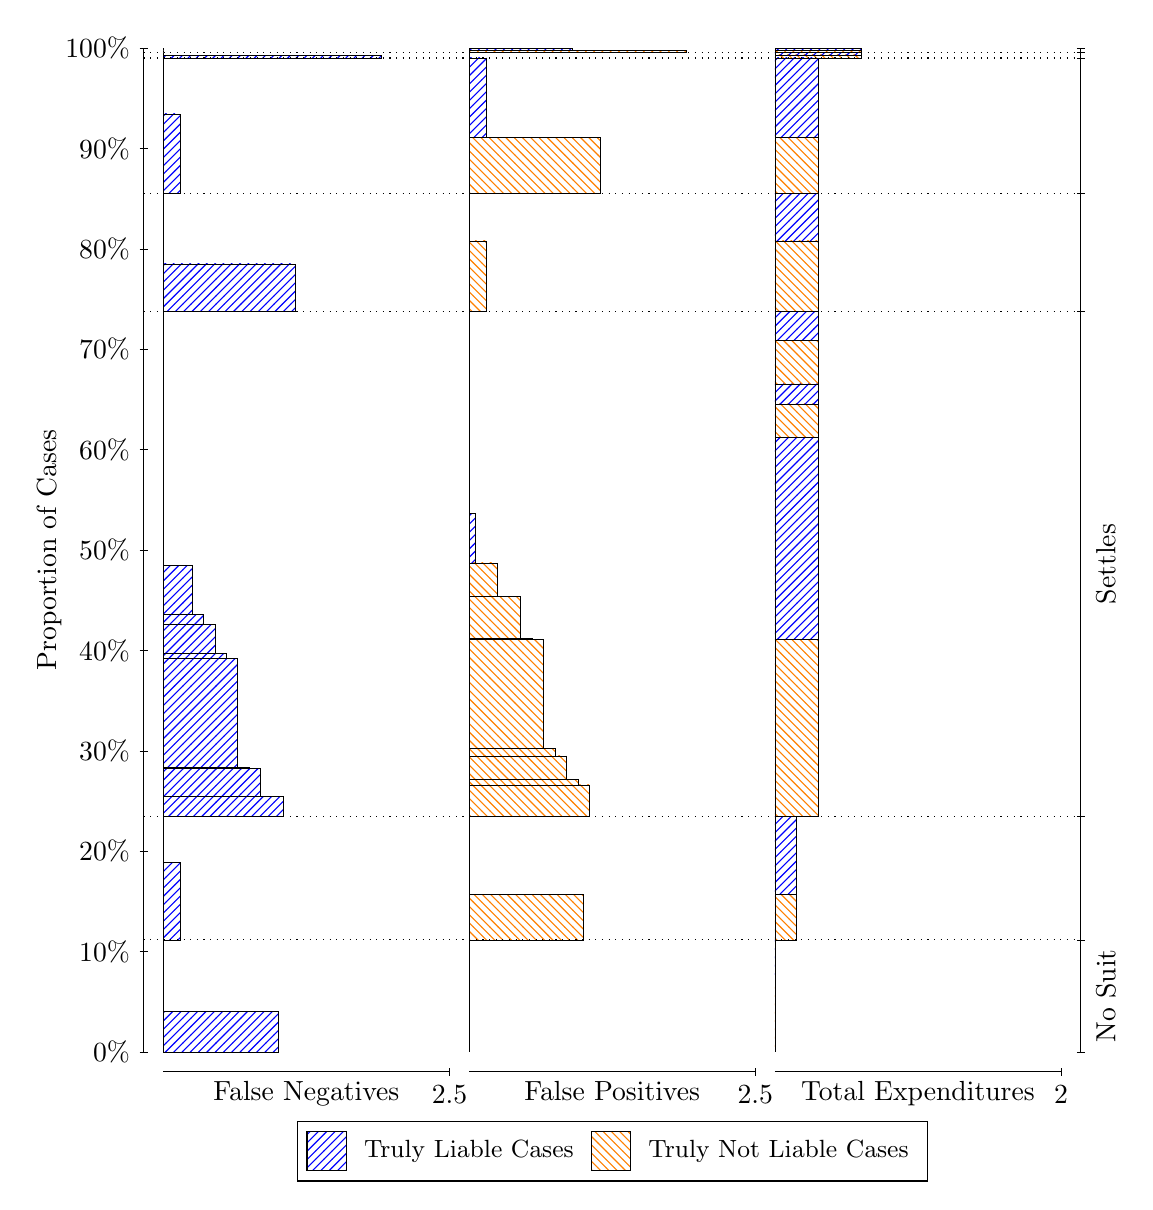
\begin{tikzpicture}
\draw[black, very thin] (1.5,1.75) -- (1.5,14.5);
\node[rotate=90, text=black, anchor=center] at (0.3, 8.125) {Proportion of Cases};
\draw[black, very thin] (1.45,1.75) -- (1.55,1.75);
\node[text=black, anchor=east] at (1.45, 1.75) {0\%};
\draw[black, very thin] (1.45,3.025) -- (1.55,3.025);
\node[text=black, anchor=east] at (1.45, 3.025) {10\%};
\draw[black, very thin] (1.45,4.3) -- (1.55,4.3);
\node[text=black, anchor=east] at (1.45, 4.3) {20\%};
\draw[black, very thin] (1.45,5.575) -- (1.55,5.575);
\node[text=black, anchor=east] at (1.45, 5.575) {30\%};
\draw[black, very thin] (1.45,6.85) -- (1.55,6.85);
\node[text=black, anchor=east] at (1.45, 6.85) {40\%};
\draw[black, very thin] (1.45,8.125) -- (1.55,8.125);
\node[text=black, anchor=east] at (1.45, 8.125) {50\%};
\draw[black, very thin] (1.45,9.4) -- (1.55,9.4);
\node[text=black, anchor=east] at (1.45, 9.4) {60\%};
\draw[black, very thin] (1.45,10.675) -- (1.55,10.675);
\node[text=black, anchor=east] at (1.45, 10.675) {70\%};
\draw[black, very thin] (1.45,11.95) -- (1.55,11.95);
\node[text=black, anchor=east] at (1.45, 11.95) {80\%};
\draw[black, very thin] (1.45,13.225) -- (1.55,13.225);
\node[text=black, anchor=east] at (1.45, 13.225) {90\%};
\draw[black, very thin] (1.45,14.5) -- (1.55,14.5);
\node[text=black, anchor=east] at (1.45, 14.5) {100\%};

\draw[black, very thin] (13.4,1.75) -- (13.4,14.5);
\draw[black, very thin] (13.35,1.75) -- (13.45,1.75);
\node[anchor=west] at (13.35, 1.75) {};
\draw[black, very thin] (13.35,3.1737) -- (13.45,3.1737);
\node[anchor=west] at (13.35, 3.1737) {};
\draw[black, very thin] (13.35,4.7386) -- (13.45,4.7386);
\node[anchor=west] at (13.35, 4.7386) {};
\draw[black, very thin] (13.35,11.153) -- (13.45,11.153);
\node[anchor=west] at (13.35, 11.153) {};
\draw[black, very thin] (13.35,12.654) -- (13.45,12.654);
\node[anchor=west] at (13.35, 12.654) {};
\draw[black, very thin] (13.35,14.374) -- (13.45,14.374);
\node[anchor=west] at (13.35, 14.374) {};
\draw[black, very thin] (13.35,14.441) -- (13.45,14.441);
\node[anchor=west] at (13.35, 14.441) {};
\draw[black, very thin] (13.35,14.5) -- (13.45,14.5);
\node[anchor=west] at (13.35, 14.5) {};

\draw[black, very thin, pattern color=blue, pattern=north east lines] (1.75,1.75) rectangle (3.2033,2.2699);
\draw[black, very thin, pattern color=orange, pattern=north west lines] (1.75,2.2699) rectangle (1.75,3.1737);
\draw[black, very thin, pattern color=blue, pattern=north east lines] (1.75,3.1737) rectangle (1.968,4.1608);
\draw[black, very thin, pattern color=orange, pattern=north west lines] (1.75,4.1608) rectangle (1.75,4.7386);
\draw[black, very thin, pattern color=blue, pattern=north east lines] (1.75,4.7386) rectangle (3.276,4.9924);
\draw[black, very thin, pattern color=blue, pattern=north east lines] (1.75,4.9924) rectangle (2.9853,5.3503);
\draw[black, very thin, pattern color=blue, pattern=north east lines] (1.75,5.3503) rectangle (2.84,5.3615);
\draw[black, very thin, pattern color=blue, pattern=north east lines] (1.75,5.3615) rectangle (2.6947,6.7458);
\draw[black, very thin, pattern color=blue, pattern=north east lines] (1.75,6.7458) rectangle (2.5493,6.812);
\draw[black, very thin, pattern color=blue, pattern=north east lines] (1.75,6.812) rectangle (2.404,7.1806);
\draw[black, very thin, pattern color=blue, pattern=north east lines] (1.75,7.1806) rectangle (2.2587,7.303);
\draw[black, very thin, pattern color=blue, pattern=north east lines] (1.75,7.303) rectangle (2.1133,7.9316);
\draw[black, very thin, pattern color=orange, pattern=north west lines] (1.75,7.9316) rectangle (1.75,11.153);
\draw[black, very thin, pattern color=blue, pattern=north east lines] (1.75,11.153) rectangle (3.4213,11.758);
\draw[black, very thin, pattern color=orange, pattern=north west lines] (1.75,11.758) rectangle (1.75,12.654);
\draw[black, very thin, pattern color=blue, pattern=north east lines] (1.75,12.654) rectangle (1.968,13.663);
\draw[black, very thin, pattern color=orange, pattern=north west lines] (1.75,13.663) rectangle (1.75,14.374);
\draw[black, very thin, pattern color=blue, pattern=north east lines] (1.75,14.374) rectangle (4.5113,14.403);
\draw[black, very thin, pattern color=orange, pattern=north west lines] (1.75,14.403) rectangle (1.75,14.441);
\draw[black, very thin, pattern color=orange, pattern=north west lines] (1.75,14.441) rectangle (1.75,14.468);
\draw[black, very thin, pattern color=blue, pattern=north east lines] (1.75,14.468) rectangle (1.75,14.5);
\draw[black, very thin, pattern color=orange, pattern=north west lines] (5.6333,1.75) rectangle (5.6333,2.6538);
\draw[black, very thin, pattern color=blue, pattern=north east lines] (5.6333,2.6538) rectangle (5.6333,3.1737);
\draw[black, very thin, pattern color=orange, pattern=north west lines] (5.6333,3.1737) rectangle (7.0867,3.7515);
\draw[black, very thin, pattern color=blue, pattern=north east lines] (5.6333,3.7515) rectangle (5.6333,4.7386);
\draw[black, very thin, pattern color=orange, pattern=north west lines] (5.6333,4.7386) rectangle (7.1593,5.143);
\draw[black, very thin, pattern color=orange, pattern=north west lines] (5.6333,5.143) rectangle (7.014,5.2126);
\draw[black, very thin, pattern color=orange, pattern=north west lines] (5.6333,5.2126) rectangle (6.8687,5.5117);
\draw[black, very thin, pattern color=orange, pattern=north west lines] (5.6333,5.5117) rectangle (6.7233,5.6023);
\draw[black, very thin, pattern color=orange, pattern=north west lines] (5.6333,5.6023) rectangle (6.578,6.9859);
\draw[black, very thin, pattern color=orange, pattern=north west lines] (5.6333,6.9859) rectangle (6.4327,6.9981);
\draw[black, very thin, pattern color=orange, pattern=north west lines] (5.6333,6.9981) rectangle (6.2873,7.5354);
\draw[black, very thin, pattern color=orange, pattern=north west lines] (5.6333,7.5354) rectangle (5.9967,7.9604);
\draw[black, very thin, pattern color=blue, pattern=north east lines] (5.6333,7.9604) rectangle (5.706,8.5889);
\draw[black, very thin, pattern color=blue, pattern=north east lines] (5.6333,8.5889) rectangle (5.6333,11.153);
\draw[black, very thin, pattern color=orange, pattern=north west lines] (5.6333,11.153) rectangle (5.8513,12.05);
\draw[black, very thin, pattern color=blue, pattern=north east lines] (5.6333,12.05) rectangle (5.6333,12.654);
\draw[black, very thin, pattern color=orange, pattern=north west lines] (5.6333,12.654) rectangle (7.3047,13.365);
\draw[black, very thin, pattern color=blue, pattern=north east lines] (5.6333,13.365) rectangle (5.8513,14.374);
\draw[black, very thin, pattern color=orange, pattern=north west lines] (5.6333,14.374) rectangle (5.6333,14.412);
\draw[black, very thin, pattern color=blue, pattern=north east lines] (5.6333,14.412) rectangle (5.6333,14.441);
\draw[black, very thin, pattern color=orange, pattern=north west lines] (5.6333,14.441) rectangle (8.3947,14.468);
\draw[black, very thin, pattern color=blue, pattern=north east lines] (5.6333,14.468) rectangle (6.9413,14.5);
\draw[black, very thin, pattern color=orange, pattern=north west lines] (9.5167,1.75) rectangle (9.5167,2.6538);
\draw[black, very thin, pattern color=blue, pattern=north east lines] (9.5167,2.6538) rectangle (9.5167,3.1737);
\draw[black, very thin, pattern color=orange, pattern=north west lines] (9.5167,3.1737) rectangle (9.7892,3.7515);
\draw[black, very thin, pattern color=blue, pattern=north east lines] (9.5167,3.7515) rectangle (9.7892,4.7386);
\draw[black, very thin, pattern color=orange, pattern=north west lines] (9.5167,4.7386) rectangle (10.062,6.9859);
\draw[black, very thin, pattern color=blue, pattern=north east lines] (9.5167,6.9859) rectangle (10.062,9.556);
\draw[black, very thin, pattern color=orange, pattern=north west lines] (9.5167,9.556) rectangle (10.062,9.981);
\draw[black, very thin, pattern color=blue, pattern=north east lines] (9.5167,9.981) rectangle (10.062,10.235);
\draw[black, very thin, pattern color=orange, pattern=north west lines] (9.5167,10.235) rectangle (10.062,10.784);
\draw[black, very thin, pattern color=blue, pattern=north east lines] (9.5167,10.784) rectangle (10.062,11.153);
\draw[black, very thin, pattern color=orange, pattern=north west lines] (9.5167,11.153) rectangle (10.062,12.05);
\draw[black, very thin, pattern color=blue, pattern=north east lines] (9.5167,12.05) rectangle (10.062,12.654);
\draw[black, very thin, pattern color=orange, pattern=north west lines] (9.5167,12.654) rectangle (10.062,13.365);
\draw[black, very thin, pattern color=blue, pattern=north east lines] (9.5167,13.365) rectangle (10.062,14.374);
\draw[black, very thin, pattern color=orange, pattern=north west lines] (9.5167,14.374) rectangle (10.607,14.412);
\draw[black, very thin, pattern color=blue, pattern=north east lines] (9.5167,14.412) rectangle (10.607,14.441);
\draw[black, very thin, pattern color=orange, pattern=north west lines] (9.5167,14.441) rectangle (10.607,14.468);
\draw[black, very thin, pattern color=blue, pattern=north east lines] (9.5167,14.468) rectangle (10.607,14.5);
\draw[black, dotted] (1.5,3.1737) -- (13.4,3.1737);
\draw[black, dotted] (1.5,4.7386) -- (13.4,4.7386);
\draw[black, dotted] (1.5,11.153) -- (13.4,11.153);
\draw[black, dotted] (1.5,12.654) -- (13.4,12.654);
\draw[black, dotted] (1.5,14.374) -- (13.4,14.374);
\draw[black, dotted] (1.5,14.441) -- (13.4,14.441);
\draw[black, very thin] (1.75,1.5) -- (5.3833,1.5);
\node[text=black, anchor=north] at (3.5667, 1.5) {False Negatives};
\draw[black, very thin] (5.3833,1.45) -- (5.3833,1.55);
\node[text=black, anchor=north] at (5.3833, 1.45) {2.5};

\draw[black, very thin] (5.6333,1.5) -- (9.2667,1.5);
\node[text=black, anchor=north] at (7.45, 1.5) {False Positives};
\draw[black, very thin] (9.2667,1.45) -- (9.2667,1.55);
\node[text=black, anchor=north] at (9.2667, 1.45) {2.5};

\draw[black, very thin] (9.5167,1.5) -- (13.15,1.5);
\node[text=black, anchor=north] at (11.333, 1.5) {Total Expenditures};
\draw[black, very thin] (13.15,1.45) -- (13.15,1.55);
\node[text=black, anchor=north] at (13.15, 1.45) {2};

\node[text=black, centered, rotate=90] at (13.72, 2.4618) {No Suit};

\node[text=black, centered, rotate=90] at (13.72, 7.946) {Settles};





\draw (7.449999999999999,1.5) node[draw=none] (baseCoordinate) {};
\begin{scope}[align=center]
        \matrix[scale=0.5, draw=black, below=0.5cm of baseCoordinate, nodes={draw}, column sep=0.1cm]{
            \node[rectangle, draw, minimum width=0.5cm, minimum height=0.5cm, pattern color=blue, pattern=north east lines] {}; &
            \node[draw=none, font=\small, text=black] (B) {Truly Liable Cases}; &
            \node[rectangle, draw, minimum width=0.5cm, minimum height=0.5cm, pattern color=orange, pattern=north west lines] {}; &
            \node[draw=none, font=\small, text=black] (B) {Truly Not Liable Cases}; \\
            };
\end{scope}

\end{tikzpicture}
\end{document}